\documentclass[lettersize,journal]{IEEEtran}

\usepackage[UTF8,fontset=windows]{ctex}
\usepackage{verbatim} 
\usepackage{graphicx}
\usepackage{booktabs}
\usepackage{pgf-pie}
\usepackage{hyperref}
\usepackage{tikz}
\usetikzlibrary{positioning, shapes.multipart, fit, arrows.meta}
\usepackage{subcaption}
\usepackage{multirow}
\usepackage{url}
\usepackage{orcidlink}
\usepackage{xurl}
\usepackage{mdframed}
\usepackage{listings}
\usepackage{xcolor}
\usepackage{algorithm}
\usepackage{amsmath}
\usepackage{bm}
\usepackage{algorithm} % For the floating algorithm environment
\usepackage[noend]{algpseudocode} % For pseudocode commands
\usepackage{xspace}
\usepackage{listings, xcolor}
\usepackage{enumitem}
\usepackage{microtype}
\usepackage{booktabs}
\usepackage{makecell}
\usepackage{varwidth}
\usepackage{amssymb}
\usepackage{fancyhdr}

\usepackage{siunitx}
\usepackage[capitalize]{cleveref}
\crefformat{section}{第#2#1#3节}
\Crefformat{section}{第#2#1#3节}
\crefformat{figure}{图#2#1#3}
\Crefformat{figure}{图#2#1#3}
\crefformat{table}{表#2#1#3}
\Crefformat{table}{表#2#1#3}
\crefformat{algorithm}{算法#2#1#3}
\Crefformat{algorithm}{算法#2#1#3}
\crefname{definition}{定义}{定义}
\Crefname{definition}{定义}{定义}
%\setlength{\abovedisplayskip}{2.2pt}
%\setlength{\belowdisplayskip}{2.2pt}
%\setlength{\abovecaptionskip}{2.2pt}
%\setlength{\belowcaptionskip}{2.2pt}
%\setlength{\textfloatsep}{2.2pt}
%\setlength{\floatsep}{2.2pt}
%\setlength{\intextsep}{2.2pt}
%\setlength{\dbltextfloatsep}{2.2pt}
%\setlength{\dblfloatsep}{2.2pt}
\lstdefinelanguage{Solidity}{
  keywords={function, external, payable, emit},
  keywordstyle=\color{blue}\bfseries,
  ndkeywords={},
  ndkeywordstyle=\color{darkgray}\bfseries,
  identifierstyle=\color{black},
  sensitive=false,
  comment=[l]{//},
  morecomment=[s]{/*}{*/},
  commentstyle=\color{purple}\ttfamily,
  stringstyle=\color{red}\ttfamily,
  morestring=[b]',
  morestring=[b]"
}

% Define Style
\lstset{
   language=Solidity,
   backgroundcolor=\color{white},
   extendedchars=true,
   basicstyle=\footnotesize\ttfamily,
   showstringspaces=false,
   showspaces=false,
   numbers=left,
   xleftmargin=12pt,
   numberstyle=\footnotesize,
   numbersep=7pt,
   tabsize=1,
   breaklines=true,
   showtabs=false,
   captionpos=b
}

\renewcommand{\abstractname}{摘 要}
\renewcommand{\figurename}{图}
\renewcommand{\tablename}{表}
\floatname{algorithm}{算法}

\newcommand{\liuye}[1]{\textcolor{red}{Ye: #1}}

\renewcommand{\paragraph}[1]{\vskip 0.05in \noindent\textbf{#1.}}

\ifCLASSOPTIONcompsoc

  \usepackage[nocompress]{cite}
\else
  \usepackage{cite}
\fi


\ifCLASSINFOpdf

\else

\fi


\hyphenation{op-tical net-works semi-conduc-tor}
\newcommand{\tool}[0]{\textsc{PEventCatcher}\xspace}
\newcommand{\cnpaperheader}{幻影事件：揭示区块链日志伪造问题}

\fancypagestyle{fancy}{
  \fancyhf{}
  \fancyhead[L]{
\includegraphics[height=0.6cm]{dhu-logo.png}}
  \fancyhead[R]{\zihao{-5}\cnpaperheader}
  \fancyfoot[C]{\zihao{-5}\rmfamily\thepage}
  \renewcommand{\headrulewidth}{0.75pt}
  \renewcommand{\footrulewidth}{0pt}
}
\fancypagestyle{plain}{
  \fancyhf{}
  \fancyhead[L]{
\includegraphics[height=0.6cm]{dhu-logo.png}}
  \fancyhead[R]{\zihao{-5}\cnpaperheader}
  \fancyfoot[C]{\zihao{-5}\rmfamily\thepage}
  \renewcommand{\headrulewidth}{0.75pt}
  \renewcommand{\footrulewidth}{0pt}
}
\setlength{\headheight}{21pt}
\setlength{\headsep}{8pt}
\pagestyle{fancy}

\begin{document}

\title{幻影事件：揭示区块链日志伪造问题}

\author{
    Yixuan Liu$^{\orcidlink{0009-0006-2255-7901}}$, 
    Yuxin Dong$^{\orcidlink{0009-0003-6239-4690}}$,
    Ye Liu$^{\orcidlink{0000-0001-6709-3721}}$,
    Xiapu Luo$^{\orcidlink{0000-0002-9082-3208}}$,~\IEEEmembership{IEEE 高级会员,}
    和 Yi Li$^{\orcidlink{0000-0003-4562-8208}}$,~\IEEEmembership{IEEE 会员} \thanks{Yixuan Liu 和 Yi Li 就职于新加坡南洋理工大学计算与数据科学学院。}
    \thanks{Yuxin Dong 就职于中国北京大学软件与微电子学院。}
    \thanks{Ye Liu 就职于新加坡管理大学计算与信息系统学院。}
    \thanks{Xiapu Luo 就职于中国香港理工大学计算学系。}
    
}
%\author{\IEEEauthorblockN{Michael Shell}
%\IEEEauthorblockA{School of Electrical and\\Computer Engineering\\
%Georgia Institute of Technology\\
%Atlanta, Georgia 30332--0250\\
%Email: http://www.michaelshell.org/contact.html}
%\and
%\IEEEauthorblockN{Homer Simpson}
%\IEEEauthorblockA{Twentieth Century Fox\\
%Springfield, USA\\
%Email: homer@thesimpsons.com}
%\and
%\IEEEauthorblockN{James Kirk\\ and Montgomery Scott}
%\IEEEauthorblockA{Starfleet Academy\\
%San Francisco, California 96678-2391\\
%Telephone: (800) 555--1212\\
%Fax: (888) 555--1212}}

\maketitle
\thispagestyle{fancy}

\begin{abstract}
随着区块链技术的快速发展，交易日志在去中心化交易所、钱包、跨链桥以及其他第三方服务等各类应用中发挥着核心作用。然而，这些日志，尤其是基于智能合约事件的日志，极易受到操纵和伪造，从而在整个生态系统中造成严重的安全风险。针对这一问题，本文首次对基于 EVM 的区块链中的交易日志伪造现象进行了深入的安全分析，并将这一现象称为幻影事件（Phantom Events）。我们系统地建模了五类攻击，并提出了一种用于检测智能合约中事件伪造漏洞的工具。实验评估表明，在识别潜在幻影事件方面，本文方法优于现有工具。此外，我们还在多个去中心化应用中成功识别出了全部五类攻击的真实案例。最后，我们呼吁社区开发者采取积极措施，以应对这些关键安全漏洞。
\end{abstract}


\IEEEpeerreviewmaketitle


\section{引言}
\label{Sec:Introduction}

区块链是一种去中心化的数字账本技术，能够在多台计算机之间安全地记录和验证交易，从而保障数据完整性和透明性~\cite{bitcoin}。作为区块链生态系统中最具代表性的代币，比特币（Bitcoin，BTC）在 2024 年 11 月达到了 1.8 万亿美元的显著市值，体现了该技术的影响力与成功~\cite{coinmarketcap}。


在区块链技术的基础上，去中心化应用（Decentralized Applications，DApps）已成为一项关键创新~\cite{buterin2014next}。这些应用运行在部署于以太坊（Ethereum）、Polygon、Binance Smart Chain（BSC）等不同区块链网络上的智能合约之上。DApp 的扩展反映了应用开发向去中心化模式转变的趋势，并提供了去中心化金融（Decentralized Finance，DeFi）和 GameFi 等多样化服务。加密货币钱包、区块链浏览器等广泛基础设施支撑着这一持续演进的生态系统，并共同推动了区块链领域的发展活力~\cite{tang2022blockchain}。

智能合约事件和交易日志对于追踪区块链应用中的操作至关重要，它们支撑着跨链桥、钱包以及 NFT 市场等场景中的多种功能。伪造这些日志会削弱系统安全性，导致资产盗窃、欺诈以及互操作性问题，进而威胁用户信任。尽管已有研究考察了特定领域中的漏洞，例如跨链桥~\cite{Xscope,liao2024smartaxe,wang2024xguard}、NFT 所有权~\cite{sleepminting}、代码不一致性~\cite{doccon}以及代币行为~\cite{TokenScope}，但目前仍缺乏面向多类应用的事件伪造综合研究。本文通过引入\emph{幻影事件（Phantom Events）}这一新型漏洞类别来弥补上述空白，该类别揭示了区块链中\emph{日志伪造}的广泛风险。不同于以往针对孤立场景的研究，本文系统总结了去中心化应用中的事件误用现象，并探索了用于识别幻影事件的不同检测方法。在已有研究中，XScope~\cite{Xscope} 和 XGuard~\cite{wang2024xguard} 等检测工具在源代码层面运行，当仅有字节码可用时，其检测能力会受到限制。相反，SmartAxe~\cite{liao2024smartaxe} 和 TokenScope~\cite{TokenScope} 虽然分析字节码，但仅依赖字节码的方法会遗漏事件参数细节。Guidi 等人~\cite{sleepminting}的方法仅关注交易日志，由于上下文分析有限，因而存在较高误报率。我们的工具结合了字节码、源代码（若可用）以及交易数据，能够跨多类漏洞进行综合检测，同时降低单层分析方法中常见的误报问题。

幻影事件是区块链系统中的一种隐蔽操纵，它会将正常的合约事件转化为执行未授权行为的隐藏通道。这类事件会破坏区块链交易中的信任基础，使攻击者能够绕过常规安全检查实施未授权活动。它们通过模仿或轻微篡改智能合约事件，误导事件监听器、用户界面以及区块链分析工具。此类漏洞利用会破坏数据完整性，并可能造成严重的经济损失和声誉损害。例如，2024 年 2 月 9 日，攻击者通过伪造转账事件造成了 104 万美元的损失~\cite{zero_transfer}。

本文研究重点在于理解并归类不同类型的幻影事件。我们对近期区块链安全报告和文章进行了全面调研，以收集利用幻影事件相关漏洞的真实攻击案例。此外，我们审计了多个活跃智能合约，并构建了一个用于处理区块链事件的安全模型（\cref{sec:threat}），该模型是分析和归类所收集攻击场景的基础（\cref{sec:vector}）。进一步地，我们开发了一个名为 \tool 的工具，用于检测与幻影事件相关的漏洞（\cref{sec:detection}）。\tool 的设计面临多项挑战：（1）许多合约仅以字节码形式存在，缺乏事件语义，从而增加了分析难度；（2）幻影事件会模仿合法事件的格式，因此难以区分；（3）判断是否存在异常还需要理解合约的业务逻辑。

利用所提出的安全模型和检测工具，我们在多种区块链应用中识别出了大量漏洞和潜在风险（详见\cref{sec:evaluation}）。结果表明，幻影事件漏洞具有广泛分布性，并影响区块链生态系统中的多类应用。通过审计工作，我们发现了此前未被报告的不一致日志记录漏洞实例，在这些实例中，链上问题会导致链下记录出现差异。此外，我们的工具还识别出了此前未被检测到的链上历史事件问题，凸显了该工具在发现既往事件方面的有效性。在合约级分析中，我们的工具优于现有解决方案，在检测幻影事件漏洞方面表现出更高的准确性。进一步地，我们在加密货币钱包、区块链浏览器和跨链桥等多个真实应用中识别出了安全问题，并将这些发现报告给项目团队，通过负责任披露申请漏洞赏金。最后，我们在\cref{sec:mitigation}中提出了应对这些漏洞的缓解策略。

简而言之，本文的主要贡献如下：
\begin{itemize}
\item \textbf{新颖的攻击分类。}
我们较早地对区块链交易日志伪造相关攻击进行了系统分析和分类。本文提出了一个能够刻画五类攻击的安全模型。我们还识别出了此前未被报告的不一致日志记录漏洞，其中链上问题会导致链下记录出现差异。
\item \textbf{高效的检测方法。}
我们开发了一种检测机制，在识别幻影事件方面超过了现有工具，并成功发现了此前未被报告的攻击交易。
\item \textbf{实践意义。}
我们在区块链浏览器、加密货币钱包、GameFi、DeFi 和 NFT 市场等多种区块链应用中识别出了真实问题。值得注意的是，我们在一个跨链中继器中发现了漏洞，而该中继器也被其他项目使用，其中包括一个市值超过 2.5 亿美元的项目。截至目前，我们已向项目团队和漏洞赏金平台报告了六个加密货币钱包问题、一个区块链浏览器问题以及一个跨链桥问题，其中五个已被确认、一个已被修复，并通过负责任披露获得了总计 600 美元的赏金。
\end{itemize}

\section{背景}\label{sec:Background}

\subsection{基于 EVM 的区块链中的智能合约事件与交易日志}
智能合约通常由 Solidity~\cite{Solidity} 和 Vyper~\cite{Vyper} 等高级语言编写，并被编译为字节码，以便在以太坊虚拟机（Ethereum Virtual Machine，EVM）上执行~\cite{EVM}。基于 EVM 的区块链支持从简单转账到复杂 DApp 的广泛功能~\cite{DApp}。在这些区块链中，\textit{事件}和\textit{交易日志}实现了智能合约与外部系统之间的通信。当智能合约发出事件时，该事件会被记录为交易日志，其关键组成部分如下。

\paragraph{事件}
以 \texttt{Deposit} 为例，事件可被定义为一个元组 $E_{\texttt{Deposit}}(P_1, P_2, \ldots, P_n)$，其中参数 $P_i$ 可以是\textit{索引参数}（存储在\textit{主题}中），也可以是\textit{非索引参数}（存储在\textit{数据字段}中）。例如，在事件
\texttt{Deposit(address indexed account, uint256 amount, uint256 timestamp);}
中，\texttt{account} 是一个\textit{索引参数}，这意味着它会被包含在事件的主题中，从而使事件日志中的搜索和过滤更加高效。\texttt{amount} 和 \texttt{timestamp} 参数未被索引，但它们仍然提供了有关交易的重要信息。

%\liuye{Pls use detailed event declaration such as event Deposit(type indexed parameter, ...) to showcase. Otherwise, it is difficult for readers to understand what a event looks like, and what event topics and indexed parameters are.}

\paragraph{监听器}
监听器是指通过 RPC 方法订阅日志并监控特定事件的外部系统，例如 DApp 或钱包。

\paragraph{交易}
交易 $TX_{\textit{hash}}$ 表示区块链上的一次操作，例如调用智能合约中的函数 $f_{\texttt{name}}$。它包括发送方地址、接收方地址、转账金额，以及用于定义函数调用及其参数的输入数据。


\paragraph{发送者}
发送者 \( TX_{\textit{sender}} \) 是创建该交易的用户地址。

\paragraph{发出者}
发出者 $S_{\texttt{address}}$ 是在满足特定条件时触发事件的智能合约。

\paragraph{交易日志}
当智能合约执行过程中发出事件时，会生成日志 \( L_{hash} = (Topics_0^i, \allowbreak{} Data^i,\allowbreak{} S_{\texttt{address}}^i) \)。其中，\( Topics_0^i \) 表示第 \(i\) 条日志的事件签名，\( Data^i \) 包含非索引参数，\( S_{\texttt{address}}^i \) 是发出该事件的合约。这些日志存储在区块链上，并被用于事件监控。

%\liuye{Maybe we can have a unified definition for event log, e.g., event = (tx\_sender, emitter, event\_name, log\_data) and then detail each part. For me, I don't think we need to discuss much more about transaction log. We can briefly say like: a transaction may be associated with multiple event logs emitted by the called contracts. }

\subsection{代币}
在基于 EVM 的区块链中，代币以智能合约的形式实现，并遵循 \textit{ERC-20} 和 \textit{ERC-721} 等标准。这些标准定义了接口和事件，以确保不同 DApp 之间的兼容性。例如，ERC-20 规定了 \texttt{Transfer} 和 \texttt{Approval} 等事件，用于追踪代币转账和授权；而 \textit{ERC-721} 定义了类似事件，但适用于每个代币都具有唯一性的 NFT。这些标准化事件使钱包和交易所等外部系统能够监控代币活动，并实时更新用户余额或所有权记录，从而保证追踪的准确性和效率。

\begin{figure}[t]
    \centering
    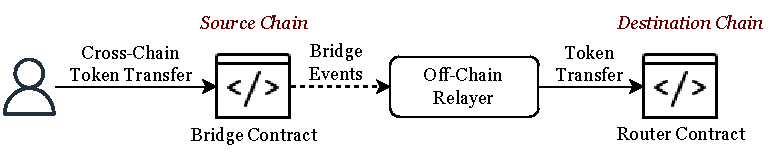
\includegraphics[width=\linewidth]{Sections/Picture/bridge.pdf}
    \caption{跨链桥的基本架构。}
    \label{fig:Bridge}
\end{figure}

\subsection{跨链桥}
一些 DApp 依赖链下模块来监控智能合约发出的交易和事件，以便实时获知链上活动和状态变化。例如，跨链桥会利用这些事件触发链下流程、更新用户界面或执行其他操作。

以跨链桥为例，如\cref{fig:Bridge}所示，\emph{源链}上的智能合约作为发出者 $S_{source}$，会在用户存入资产时发出 \texttt{Deposit} 等特定事件。而\emph{目标链}上的智能合约则作为执行方，由链下中继器调用，用于处理已存入的资产并完成转账操作。

当用户在源链上的\emph{桥合约}中存入代币时，会发出存款事件 $E_{\texttt{Deposit}}$，并将其记录为交易日志 $L_{deposit_{tx}}$。\emph{链下中继器}作为监听器，会监控这些日志以检测 \texttt{Deposit} 事件，处理事件信息，并与目标链上的智能合约协同完成资产转移。

\section{威胁模型与动机示例}\label{sec:threat}

本节提出一个用于系统分析事件相关攻击的威胁模型，并通过动机示例说明幻影事件的影响。
\subsection{事件交互中的信任边界}

在复杂的区块链交互环境中，建立清晰的信任边界对于全面理解交易与事件工作流中的安全风险和漏洞至关重要。\cref{fig:system model}所示的交互模型定义了三个主要信任边界：
\begin{figure}[t]
    \centering
    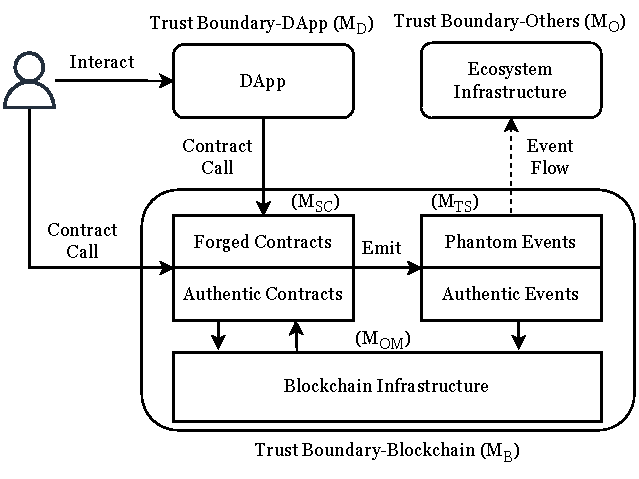
\includegraphics[width=.9\linewidth]{Sections/Picture/securitymodel.pdf}
    \caption{区块链交互中的信任边界}
    \label{fig:system model}
\end{figure}

\paragraph{信任边界-区块链（\(\bm{\mathcal{M}}_B\)）}
核心信任边界是区块链，它作为系统的基础支撑，用于存储交易和智能合约事件。
该边界内包含交易存储（\(\bm{\mathcal{M}}_{TS}\)），可进一步划分为\emph{幻影事件}和\emph{真实事件}。
幻影事件是人为创建或操纵的事件，可能触发非预期操作；真实事件则是区块链交易的预期输出。
智能合约区域（\(\bm{\mathcal{M}}_{SC}\)）可划分为\emph{真实合约}和\emph{伪造合约}，分别表示合约按预期运行或恶意运行的可能性。
其他区块链模块（\(\bm{\mathcal{M}}_{OM}\)）包括共识机制、节点通信协议以及其他支撑区块链功能的组件。

\paragraph{信任边界-DApp（\(\bm{\mathcal{M}}_{D}\)）}
第二个边界涵盖作为用户与区块链之间接口的 DApp。
DApp 会监听来自区块链的事件并作出相应响应，通常会根据这些事件触发交易或更新。


\paragraph{信任边界-其他组件（\(\bm{\mathcal{M}}_{O}\)）}
第三个边界包括更广泛的生态系统，例如链下服务、外部 API 和钱包。这些组件同样依赖区块链事件的完整性来保证其功能正常运行。

\subsection{威胁模型}
在我们的威胁模型中，攻击者试图通过发出伪造事件来破坏 DApp 及更广泛的生态基础设施，也可能利用这些攻击并结合社会工程学手段误导用户。普通用户通过调用真实合约发出合法事件，而攻击者可以通过多种方式发出伪造事件：调用伪造合约、调用真实合约，或调用一个随后再调用真实合约的伪造合约以发出伪造事件。攻击者的能力被限定为直接进行合约调用或与 DApp 交互。

\subsection{动机示例}\label{sec:motivation}
现实中已经发生了大量由交易日志伪造导致的区块链攻击。
例如，Qubit Bridge 和 pNetwork Bridge 攻击~\cite{Qubit,pNetwork}均利用了幻影事件漏洞，分别造成了 8000 万美元和 430 万美元的损失。

\begin{figure}[h]
    \centering
    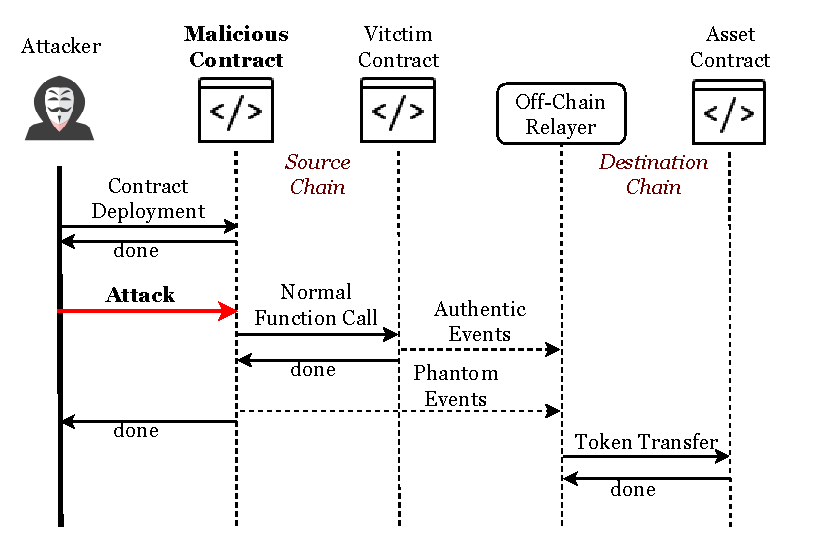
\includegraphics[width=1\columnwidth]{Sections/Picture/sequencediagram.pdf}
    \caption{pNetwork 攻击的攻击序列。}
    \label{fig:sqeuence}
\end{figure}

在 pNetwork 攻击中，事件处理机制存在缺陷：如果恶意合约和合法合约在同一笔交易中均被调用并发出事件，该机制会错误地将所有发出的事件都视为合法合约事件。因此，如攻击序列（\cref{fig:sqeuence}）所示，攻击者首先在源链上部署了恶意合约 $S_{\texttt{malicious}}$，该合约通过函数调用来调用合法合约 $S_{\texttt{legitimate}}$。在合法合约 $S_{\texttt{legitimate}}$ 执行其函数 $f_{\texttt{deposit}}$ 并发出真实事件 $E_{\texttt{Deposit}}$ 后，恶意合约 $S_{\texttt{malicious}}$ 同时发出了一个金额不真实的伪造事件 $E_{\texttt{Deposit}}$。由于真实事件和伪造事件都被记录在同一笔交易 $TX_{\textit{deposit}}$ 下，中继器便像处理合法事件一样处理了该伪造事件。攻击者由此利用系统无法区分这两个事件的缺陷，将未授权资金转移到目标链。

在 Qubit Bridge 攻击中，攻击者利用了受害合约 \texttt{deposit} 函数中的缺陷，如\cref{code:1}所示。中继器通过从源链发出的事件中获取代币地址和数量，并据此在目标链上转移资产。然而，攻击者利用 \texttt{deposit} 函数发出了本应仅由 \texttt{depositETH} 函数发出的事件，使其能够在源链上并未实际存入任何 ETH 的情况下，触发目标链上的 ETH 转账，从而绕过中继器检查并从攻击中获利。


\begin{comment}
Another example is the transfer spoofing attack on 9 February 2024, where an attacker successfully executed a \textit{transfer event spoofing} attack, resulting in a loss of \$1.04 million USD. This attack exploited vulnerabilities in wallets and blockchain explorers that parse and display transfer events. As shown in~\Cref{tab:transfer_spoof_attack_transaction}, after a user sent funds to a legitimate address (0x734\ldots{}a79F7), the attacker forged a transfer event, making it appear as though the funds were sent to a similar address controlled by the attacker. Due to the way certain wallets and explorers processed these events, the fake transfer was displayed as legitimate, leading the user to mistakenly send additional funds to the attacker's address, resulting in significant financial losses~\cite{zero_transfer}.
\end{comment}
\paragraph{\tool 的设计思路}
受这些真实案例启发，我们针对不同类型的漏洞采用了定制化检测方法。幻影事件可能源于智能合约逻辑中的问题，也可能源于链下处理器中的缺陷。为此，我们设计了一种智能合约级方法，用于识别可能导致幻影事件的漏洞。此外，我们还为交易数据开发了一种链上方法，通过检查交易中的模式或异常来判断其是否可能表明攻击。这些方法相互补充，使检测框架能够同时覆盖幻影事件中基于合约和基于交易的成因。

\section{攻击分类与分析}\label{sec:vector}

本节给出由幻影事件导致的攻击分类，并为每类攻击提供详细解释和检测规则。

\begin{table*}[ht]
\centering
\caption{攻击向量与相关模块之间的映射关系。}
\label{tab:attack-classification}
\begin{tabular}{l|l|p{8.5cm}|p{3cm}}
\toprule
\textbf{层级} & \textbf{攻击} & \textbf{描述} & \textbf{相关模块} \\
\midrule
\multirow{2}{*}{\textbf{链上}}
& 事件仿冒 & 利用现有合约发出幻影事件 & \(\bm{\mathcal{M}}_{TS}\), \(\bm{\mathcal{M}}_{O}\) \\
\cmidrule{2-4}
& 不一致日志记录 & 数据库记录与区块链事件发出之间存在不一致 & \(\bm{\mathcal{M}}_{SC}\), \(\bm{\mathcal{M}}_{TS}\), \(\bm{\mathcal{M}}_{D}\) \\
\midrule
\multirow{3}{*}{\textbf{链下}}
&合约仿冒 & 部署恶意合约以发出幻影事件 & \(\bm{\mathcal{M}}_{SC}\), \(\bm{\mathcal{M}}_{TS}\), \(\bm{\mathcal{M}}_{O}\) \\
\cmidrule{2-4}
& 转账事件欺骗 & 结合社会工程学攻击发出幻影事件 & \(\bm{\mathcal{M}}_{SC}\), \(\bm{\mathcal{M}}_{TS}\), \(\bm{\mathcal{M}}_{O}\) \\
\cmidrule{2-4}
& 事件处理错误 & 由于事件处理存在缺陷而导致错误显示、插入或存储 & \(\bm{\mathcal{M}}_{D}\), \(\bm{\mathcal{M}}_{O}\) \\
\bottomrule
\end{tabular}
\end{table*}

我们基于行业报告、学术文献以及真实世界中的智能合约审计，构建了一个针对相对新颖且研究不足的幻影事件攻击的分类体系。我们建模了五种不同的攻击场景，并根据其来源将其划分为两类：（1）\emph{链上（智能合约）漏洞}；（2）\emph{链下弱点}。这些攻击总结于攻击分类表（\cref{tab:attack-classification}）中。

这些攻击的详细演示可见补充材料。\footnote{\url{https://github.com/PhantomEvent/Event-attack-demo}}


\subsection{攻击向量与检测规则}
本节介绍五种与幻影事件相关的攻击，并提出相应的检测规则。这些攻击的示例见\cref{appendix:examples}。

\subsubsection{事件仿冒}\label{vec:attack1}

\begin{figure}
\small
\footnotesize
\begin{lstlisting}[language=Solidity]
function depositETH(uint destinationChainId) external payable {
  require(msg.value > 0, "Deposit amount must be greater than 0");
  ethBalances[msg.sender] += msg.value;
  emit Deposit(msg.sender, msg.value, address(0), destinationChainId);
}

function deposit(address token, uint amount, uint destinationChainId) external {
  require(amount > 0, "Deposit amount must be greater than 0");
  safeTransfer(token, address(this), amount);
  tokenBalances[msg.sender][token] += amount;
  emit Deposit(msg.sender, amount, token, destinationChainId);
}

function safeTransfer(address token, address to, uint value) internal {
  (bool success, bytes memory data) = token.call(abi.encodeWithSelector(0xa9059cbb, to, value));
  require(success && (data.length == 0 || abi.decode(data, (bool))), "!safeTransfer");
}
\end{lstlisting}
\caption{事件仿冒攻击的概念验证，其中 \texttt{deposit} 和
\texttt{depositETH} 可能发出相同事件。}\label{code:1}
\end{figure}

该攻击利用合法合约中多个函数或执行路径会发出相同事件这一特性（\(\bm{\mathcal{M}}_{TS}\)）。在\cref{code:1}所示的代码示例中，\texttt{depositETH} 和 \texttt{deposit} 函数都会发出 \texttt{Deposit} 事件，其中第三个参数表示代币类型。\texttt{depositETH} 使用 \texttt{address(0)} 表示 ETH，而 \texttt{deposit} 函数则使用代币地址表示 ERC-20 代币。然而，\texttt{deposit} 函数也可以发出第三个参数为 \texttt{address(0)} 的事件，从而模仿一次 ETH 存款。

攻击者可以通过调用 \texttt{deposit} 函数并将第三个参数伪造为 \texttt{address(0)} 来利用这一点，而无需实际转移任何 ETH。这会创建一个类似真实 ETH 存款的\emph{幻影} \texttt{Deposit} 事件。依赖事件日志进行交易验证的链下验证系统可能会错误地将该事件视为合法的 ETH 存款。由于事件验证流程存在缺陷，攻击者便能够在目标链上欺诈性地申领大量资产。


\paragraph{检测方法}
当不同函数或执行路径以相同参数发出同一事件，而这些函数本应施加不同约束时，就会出现该漏洞。链下系统通常会在未验证参数约束的情况下将这些事件视为真实事件。如果某个函数发出了一个本应由另一个函数约束或验证的值，则可将其视为潜在漏洞。检测规则会检查不同执行路径是否发出了相同参数值，即使这些路径原本应强制执行不同约束；若满足该条件，则将此类事件标记为潜在漏洞。


形式化检测规则表示如下。

\begin{equation}
\small
\text{EC} = \left\{
e \in E \mid
\begin{aligned}
  & V(f, e) \cap V(g, e) \neq \emptyset \text{ and } \\
  & \exists \; f, g \in F(e)
\end{aligned}
\right\}
\end{equation}


\begin{itemize}
    \item \( E \) 是已发出事件的集合，\( e \in E \) 表示单个事件。
    \item \( F \) 是合约中所有能够发出事件的函数路径集合，\( f, g \in F \) 是发出同一事件 \( e \) 的特定函数路径。
    \item \( V(f, e) \) 和 \( V(g, e) \) 表示事件 \( e \) 的参数在函数路径 \( f \) 和 \( g \) 上可能取得的值范围。
\end{itemize}


\subsubsection{不一致日志记录}\label{vec:attack2}

\begin{figure}
\footnotesize
\small
\begin{lstlisting}[language=Solidity]
function requestWithdraw(uint256 _type, uint256 _amount) external {
  require(WITHDRAW_ALLOWED, "TroyEmpire: Withdrawal is disabled for now");
  emit WithdrawalRequested(_msgSender(), _type, _amount);
}
\end{lstlisting}
\caption{不一致日志记录攻击的概念验证。}\label{code:2}
\end{figure}

许多 DApp 采用混合日志记录模型，同时使用区块链和传统数据库记录关键操作。例如，DeFi 平台会记录存款和取款等金融交易，而 GameFi 平台会追踪用户操作。我们的分析表明，许多项目不仅依赖数据库记录，还会在区块链上发出日志。

具体而言，设计不当的智能合约可能允许攻击者发出伪造事件，从而导致区块链日志与数据库日志之间出现不一致。例如，某金融平台可能同时使用区块链和链下数据库记录取款请求。如果智能合约缺乏适当的访问控制，攻击者就可以在区块链上任意生成取款事件，进而造成其与数据库记录不匹配，如\cref{code:2}所示。


\paragraph{检测方法}
当智能合约在缺乏适当访问控制或未与已存储数据进行校验的情况下发出事件时，就会出现该漏洞。具体而言，一些合约缺少必要约束，允许任意用户触发取款等关键事件，而不根据合约状态验证事件参数。为检测该问题，我们从两个关键方面分析合约函数：（1）是否存在访问控制机制或事件参数验证（例如 \texttt{require} 语句），以限制谁可以发出事件；（2）函数在发出事件时是否与存储交互，即是否读取或写入存储变量，以确保参数经过此前存储值的验证。如果某个函数在缺乏充分访问控制的情况下发出事件，或未与存储交互，则将其标记为潜在漏洞。

形式化检测规则表示如下。

\begin{equation}
\small
\text{IL} = \left\{
f \in F \mid
\begin{aligned}
  & Constraint(f) = \emptyset \text{ or } \\
  & (S_{\texttt{read}}(f) = \emptyset \text{ and } S_{\texttt{write}}(f) = \emptyset)
\end{aligned}
\right\}
\end{equation}


\begin{itemize}
    \item \( Constraint(f) \)：函数 \( f \) 的访问控制机制或事件参数约束。如果 \( Constraint(f) = \emptyset \)，则表示不存在访问控制或约束。
    \item \( S_{\texttt{read}}(f) \) 和 \( S_{\texttt{write}}(f) \)：函数 \( f \) 读取和写入的存储变量。
\end{itemize}

\subsubsection{合约仿冒}\label{vec:attack3}

该攻击涉及部署恶意合约以利用或模仿现有合约（\(\bm{\mathcal{M}}_{SC}\)）。我们根据其特征将该攻击划分为两个子类型。第一种子类型称为混合事件攻击（Blended Event Attack），当恶意合约与合法合约交互，使两个合约发出的事件都被记录在同一笔交易中时，就会发生该攻击。这种事件混合使合法活动与欺诈活动难以区分。第二种子类型称为仿冒合约攻击（Mimicry Contract Attack），即攻击者部署一个模仿合法合约行为的伪造合约，从而操纵事件日志和交易细节。


\emph{真实}合约通常记录其自身函数产生的日志。然而，大多数合约允许外部调用，因此恶意合约可以调用其函数，导致两个合约产生的日志被记录在同一笔交易中（\(\bm{\mathcal{M}}_{TS}\)）。这一场景被称为\emph{混合事件}攻击。当日志发出者未被验证时，该攻击会引入安全风险。

\emph{仿冒合约}攻击利用了透明化实践，因为许多 DApp 团队会公开合约源代码以增强信任。这使攻击者能够修改并重新部署代码，创建模仿合法合约的恶意合约，并发出可被任意操纵的事件日志（\(\bm{\mathcal{M}}_{TS}\)）。对于 ERC-20 代币或 NFT 而言，这种操纵使攻击者能够伪造交易记录，例如铸造或转移代币或 NFT；其中还可能包括伪造发送者，使 NFT 看起来仿佛由知名艺术家发行。

\paragraph{检测方法}
%This vulnerability arises when an attacker deploys a forged contract to mimic an authentic contract, emitting phantom events that resemble legitimate ones. The attacker can further blend these phantom events with authentic events within the same transaction log, making it difficult for off-chain systems to distinguish between legitimate and forged events.
为检测该攻击，我们分析\emph{交易日志}。具体而言，我们检查相同事件签名（\( Topics_0 \)）是否在同一笔交易中多次出现，但由不同合约发出。如果同一事件签名在同一笔交易中同时由真实合约和伪造合约发出，则将其标记为潜在攻击交易。该检测规则有助于识别事件签名相同但发出者不同的情况，这表明可能存在\emph{混合事件攻击}。


\begin{equation}
\small
\text{BE} = \left\{
L_{\textit{hash}} \mid
\begin{aligned}
  & Topics_0^i = Topics_0^j \text{ and } \\
  & S_{\texttt{address}}^i = S_{\texttt{auth}} \text{ and } \\
  & S_{\texttt{address}}^j = S_{\texttt{forge}}
\end{aligned}
\right\}
\end{equation}



\subsubsection{转账事件欺骗}\label{vec:attack4}

该攻击是一种社会工程学攻击~\cite{social_engineer}。一个常见示例是零转账骗局（Zero Transfer Scam），攻击者会创建一个模仿合法代币转账的幻影事件。用户发送代币后，攻击者生成一个虚假事件，使其看起来像是用户已将代币发送至一个名称相似的接收地址，而该地址实际上由攻击者控制。这一伪造事件会被钱包和区块链浏览器记录，从而误导受害者将更多资金转入攻击者账户。据报道，该骗局已造成至少 2736 万美元的损失，并影响了 28,414 名受害者~\cite{wallet_visual}。

第二种变体称为空投骗局（Airdrop Scam）~\cite{spoof}，它利用了 Web3 中常见的代币空投营销策略。攻击者使用真实的 ERC-20 或 ERC-721 合约伪造发送者地址，从而伪造幻影事件，并且通常会选择容易吸引注意力的地址（例如 0x8888...8888）。这些幻影空投会诱骗受害者与代币交互。攻击者可能设置蜜罐合约，使用户可以买入代币但无法卖出；也可能利用幻影事件日志推广恶意链接，例如使用 ENS 名称欺骗受害者。在更严重的情况下，攻击者可能实施 rug pull，撤走流动性并使受害者持有毫无价值的代币~\cite{rugpull}。


\paragraph{检测方法}
攻击者利用了许多第三方服务（如钱包和区块链浏览器）盲目信任智能合约发出事件、却不验证其真实性这一事实。借助这种验证缺失，攻击者可以生成模仿合法转账的幻影事件，误导用户将资金转入攻击者地址。为检测该攻击，可以分析交易日志，以确保转账事件确实由正确的发送者发起，或者验证发送者是否已授权发起交易的地址转移其代币。


\begin{equation}
\small
\text{TS} = \left\{
L_{\textit{hash}} \mid
\begin{aligned}
  & TX_{\textit{sender}} \neq \textit{TokenSender} \text{ and } \\
  & Approve(\textit{TokenSender}, TX_{\textit{sender}}) = \text{false}
\end{aligned}
\right\}
\end{equation}


\begin{itemize}
    \item \( \textit{TokenSender} \) 表示事件中的代币发送者。
    \item \( Approve(\textit{TokenSender}, TX_{\textit{sender}}) \) 表示代币发送者是否已授权交易发起者转移其代币。
\end{itemize}

\subsubsection{事件处理错误}\label{vec:attack5}
该攻击利用区块链浏览器、钱包和监控工具在处理和解释交易数据时存在的漏洞。这些应用依赖链上数据向用户提供实时信息。当幻影事件被错误地视为合法事件时，可能导致钱包余额不准确、交易历史虚假或资产所有权记录错误，从而误导用户并可能影响其决策。

例如，在\emph{合约仿冒}攻击场景中，即使幻影事件并非专门针对区块链浏览器，它们仍可能导致浏览器将这些事件记录为有效的 ERC-20 或 NFT 转账，尽管实际上并未发生任何转账。这种误解使攻击者能够在不存在底层交易的情况下制造转账表象。

攻击者还可以进一步在事件数据中嵌入恶意载荷，以发起跨站脚本（cross-site scripting，XSS）或 SQL 注入（SQL injection，SQLi）等攻击。如果缺乏适当的清理与过滤，这些载荷可能导致 DApp 界面上的未授权操作、数据窃取或数据库被攻陷。

\paragraph{检测方法}
该攻击利用了区块链浏览器、钱包和监控工具对链上数据的隐式信任。有效检测需要根据各类链下应用的需求设计可适配的方法。浏览器应根据实际代币转账验证事件，而钱包需要确认发送者是否被允许执行该转账。通过基于这些特定验证标准定制检测规则，应用可以降低幻影事件和嵌入式恶意载荷带来的风险。

\section{漏洞检测}\label{sec:detection}

\begin{figure*}[t]
  \centering
  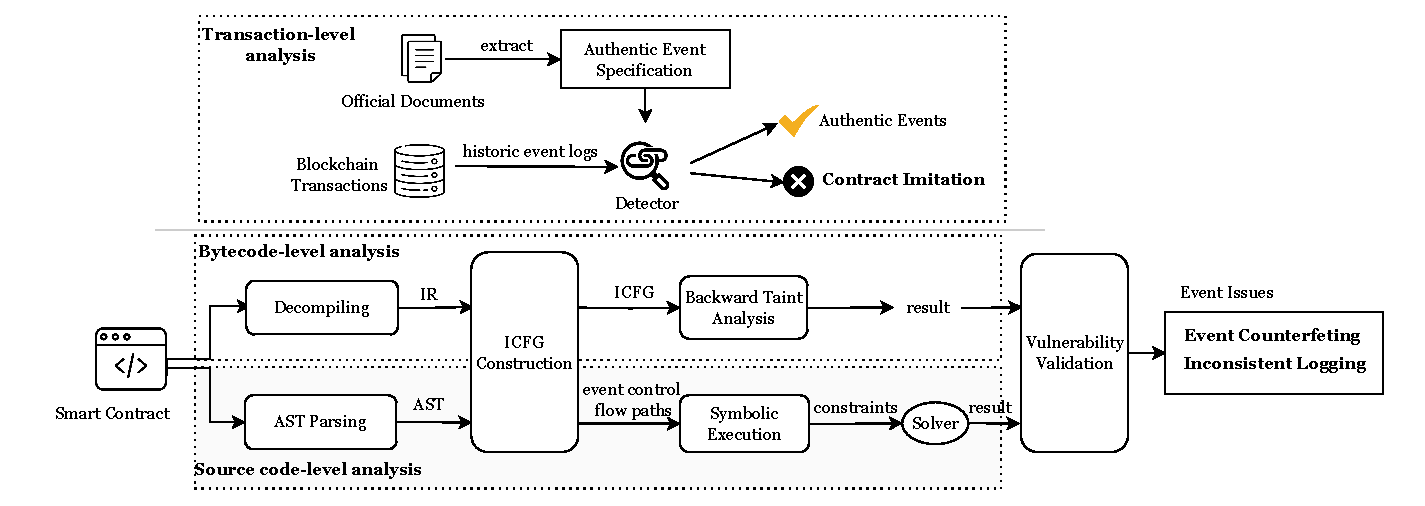
\includegraphics[width=\linewidth]{Sections/Picture/PhatomEventOverview.pdf}
  \caption{\tool 的架构。}
  \label{fig:tool}
\end{figure*}

本节重点讨论与\cref{sec:vector}中攻击向量相关的漏洞检测。我们介绍一种混合方法，该方法结合静态分析、符号执行和链上数据监控，以实现全面的漏洞检测。

\subsection{\tool 框架设计}

如\cref{fig:tool}所示，我们的检测方法采用多层级策略，覆盖交易级、字节码级和源代码级漏洞检测。

在交易级，由于不同项目中的真实事件和发出者存在差异，我们人工研究了不同项目的文档，以建立适当的规则。这些规则被应用于历史和实时链上交易数据，通过识别幻影事件与真实事件混合的实例来检测\emph{合约仿冒}。

对于智能合约，我们的分析同时覆盖字节码和源代码两个层面。首先，我们使用 Gigahorse~\cite{Gigahorse} 将智能合约字节码反编译为三地址形式的中间表示（intermediate representation，IR）。随后，基于该 IR 的基本块构建跨合约控制流图（inter-contract control flow graph，ICFG）。该图支持后向污点分析，我们利用它追踪与事件相关的路径，并检测与\emph{事件仿冒}和\emph{不一致日志记录}相关的漏洞。

如果源代码可用，我们会使用 Slither 扩展分析并执行源代码级分析。通过追踪事件相关调用路径并提取用于符号执行的约束，该分析能够对\emph{事件仿冒}进行二次确认，使我们能够更全面地验证参数值。

由于某些攻击具有特殊性质，\emph{事件处理错误}高度依赖链下系统验证，因此缺乏特定的检测方法。类似地，\emph{转账事件欺骗}主要是一类社会工程学攻击，其分析重点在于代币行为。因此，我们的工具主要针对其余三类攻击进行检测：\emph{事件仿冒}、\emph{不一致日志记录}和\emph{合约仿冒}。这些攻击具有较为明确的模式和合约级漏洞，因而能够被有效识别和处理。

\subsection{交易级检测}
在交易级，我们采用链下监控来分析链上交易数据，并检测潜在的\emph{合约仿冒}攻击。通过基于智能合约预期行为建立领域特定规则，我们系统地验证交易是否符合正确逻辑，并识别任何可能表明幻影事件或未授权交互的恶意活动迹象。

该分析涉及解析交易数据，并应用一组规则来验证事件的关键方面，包括：（1）确保发出的事件具有正确的签名；（2）验证事件发出者是否与预期合约地址匹配；（3）检查函数执行路径是否符合预期逻辑；（4）确认事件参数值是否与预期值一致。

通过执行这些规则，我们能够检测可能表明\emph{合约仿冒}攻击的异常。如果检测到攻击交易，则进一步分析其影响，例如是否造成未授权资金转移或状态变化。

\begin{table*}[t]
  \centering
  \caption{pNetwork 攻击的交易日志。}
  \label{tab:pnetwork_transaction}
  \resizebox{\textwidth}{!}{
    \begin{tabular}{lllp{7cm}}
      \toprule
      \textbf{事件} & \textbf{参数} & \textbf{发出者} & \textbf{参数值} \\
      \midrule
      Burned &
      operator, from, amount, data, operatorData &
      pBTC &
      (Attacker, Attacker, 0, , \_ ) \\
      \midrule
      Transfer &
      from, to, amount &
      pBTC &
      (Attacker, address(0), 0)\\
      \midrule
      Redeem &
      redeemer, value, underlyingAssetRecipient, userData &
      pBTC &
      (Attacker, 0, Attacker\_Bitcoin\_address, \_) \\
      \midrule
      Redeem &
      redeemer, value, underlyingAssetRecipient, userData &
      Malicious Contract &
      (Attacker, 274[...]144, Attacker\_Bitcoin\_address, \_) \\
      \bottomrule
  \end{tabular}}%
  %}
  \end{table*}

例如，在 pNetwork 攻击中（\cref{tab:pnetwork_transaction}），一个 \emph{Redeem} 事件由源链上具有非预期合约地址的恶意合约发出。应用这些交易级规则使我们能够检测到该攻击。随后对目标链交易的监控确认，该攻击通过未授权资金转移取得了成功。



\subsection{智能合约级检测}

\begin{algorithm}[t]
\label{algo:bytecode}
  \footnotesize
  \caption{通过后向污点分析检测不一致日志记录与事件仿冒}
  \textbf{输入：} \textit{IR}，通过反编译得到的智能合约字节码中间表示。 \\
  \textbf{输出：} $E_v$，漏洞事件集合。 
  \begin{algorithmic}[1]
    \State  $E_v = \emptyset$. 
    \State \textbf{construct} \textit{ICFG} out of IR.
    \State \textbf{extract} \textit{LogOps}, i.e., event log operations, from IR. \Comment{每个操作包含一个事件签名和一组日志数据变量} 
    
    % \State logBlocks $=$ extractLogBlocks(IR) \Comment{Extract log blocks with event signatures and variables}
    \State  \textit{Vars} $= \emptyset$, 
    \For{logOp $\in$ \textit{LogOps}}
      \State Vars $\gets$ Vars $\cup$ \textbf{vars}(logOp)  \Comment{记录所有日志数据变量}
      \State Slices $\gets$ \textsc{BackwardSlicing}(logOp, ICFG) \Comment{每个切片都是从 logOp 到函数入口点的反向执行流路径}
          \State \textbf{extract} \textit{Paths}, i.e., inter-functional paths based on Slices and ICFG
      \State taintedPaths $\gets \emptyset$   
      \For{$p \in$ Paths}
        \State $source_{op} \gets$ \textsc{TaintAnalysis}($p$, Vars) 
        \If{$source_{op} \neq null$}
            \If{\textbf{sstore}($p$[:$source_{op}$]) $= \emptyset$} 
                \State $E_v \gets E_v \cup \textbf{event}(logOp)$ \Comment{不存在存储操作}
            \EndIf
            \State taintedPaths $\gets taintedPaths \cup \{\textbf{event}(logOp)\} $   
        \Else
            \If{HasExternalCall($p$) $\land$ not HasJumpi($p$)}
                 \State $E_v \gets E_v \cup \textbf{event}(logOp)$ \Comment{不存在约束}
            \EndIf

        \EndIf
        % \State $src \gets$ TaintAnalysis($p$, taintVars, src) 
        
        % \If{(HasExternalCall($p$) \textbf{and not} HasJumpi($p$)) \textbf{or} (src $\neq$ null \textbf{and not} HasJumpi($p$)) \textbf{or} MultiplePathsEmitSameEvent(p, paths)}
        %   \State $Ev \gets Ev \cup \{log.event\}$ 
        % \EndIf
      \EndFor
      \If{$||taintedPaths|| >$ 1}
               \State $E_v \gets E_v \cup \textbf{event}(logOp)$ \Comment{一个事件日志记录动作具有多条污点路径}
        \EndIf
    \EndFor
    \State \textbf{return} $E_v$

\Procedure{TaintAnalysis}{path, taintVars}  
  \State $entry = path[-1]$ \Comment{函数入口点是该反向执行路径的最后一项} \label{begin:taintanalysis}
  \For{$instr \in path$}
    \If{$\textbf{vars}(instr) \cap taintVars \neq \emptyset$}
        \State taintVars $\gets$ taintVars $\cup$ $\textbf{vars}(instr)$  \Comment{污点传播}
    % \ElsIf{$instr$ == sink}
    %   \State \textbf{return} $taintVars$ \Comment{Return the tainted variable}
    \EndIf
  \EndFor

  \If{$vars(entry) \cap taintVars \neq \emptyset $}
    \State \textbf{return} entry
  \Else 
    \State \textbf{return} null  \label{end:taintanalysis}
  \EndIf 
  
\EndProcedure 

% \Procedure{TaintAnalysis}{P, taintVars}
% \State $S \gets \emptyset$ \Comment{Initialize set of source variables} \label{begin:taintanalysis}
% \For{$index \gets |P| - 1$ \textbf{down to} $0$} \Comment{Reverse traverse the instruction sequence}
%     \State $instr \gets P[index]$
%     \If{$instr.lvars \in taintVars$}
%         \State $taintVars \gets taintVars \cup instr.rvars$ 
%     \EndIf
%     \If{$instr.rvars \in taintVars$}
%         \State $taintVars \gets taintVars \cup instr.lvars$ 
%     \EndIf
% \EndFor
% \State \Return null
% \label{end:taintanalysis}
% \EndProcedure

  \end{algorithmic}
  \label{algorithm}
\end{algorithm}


在智能合约级，我们通过一种由两部分组成的多层分析方法，专门检测与\emph{事件仿冒}和\emph{不一致日志记录}相关的漏洞：（1）在字节码级通过\emph{过程间后向污点追踪}识别潜在幻影事件；（2）在源代码级通过\emph{验证事件参数约束}确认漏洞。该双方法使我们能够分析合约的不同表示形式，以识别在单一抽象层级下可能不可见的漏洞。

\subsubsection{通过过程间后向污点追踪识别幻影事件}
在字节码级，如\cref{algorithm}所述，与\emph{事件仿冒}和\emph{不一致日志记录}相关的漏洞检测，是通过对智能合约字节码的中间表示（IR）进行后向污点分析来完成的。该算法通过分析数据从事件日志操作到其来源的流动，并检查表明漏洞存在的特定条件，识别漏洞事件 \(E_v\)。

算法首先初始化一个空集合 \(E_v\)，用于存储漏洞事件（第 1 行）。随后，它从 IR 中构建过程间控制流图（ICFG）（第 2 行），并从 IR 中提取所有事件日志操作（\textit{LogOps}）（第 3 行）。每个日志操作由一个事件签名和一组事件数据变量组成。接着，算法初始化空集合 \textit{Vars} 以记录事件变量（第 4 行）。

ICFG 的构建涉及恢复函数级信息，例如函数名和事件签名，其方式是将字节码中的哈希标识符与签名数据库中的条目进行匹配。随后，使用表示每个函数内可能执行路径的基本块构建控制流图（control flow graph，CFG）。这些基本块根据控制流指令和跳转目标通过有向边连接，从而形成 CFG。为捕获跨函数交互，算法会识别过程间调用，并在调用者函数和被调用者函数之间添加边，由此将 CFG 扩展为 ICFG。

对于 \textit{LogOps} 中的每个日志操作，算法使用该日志操作涉及的变量更新 \textit{Vars}（第 6 行）。随后，它在 ICFG 上执行 \textsc{BackwardSlicing} 分析，提取表示从日志操作到函数入口点的反向执行流的切片（第 7 行）。这些切片用于推导跨函数路径（\textit{Paths}），以供进一步分析（第 8 行）。

对于 \textit{Paths} 中的每条路径 \(p\)，算法使用 \textsc{TaintAnalysis} 函数执行污点分析（第 9 行）。该函数评估污点数据是否从日志操作传播到路径入口点。污点变量从日志操作开始，通过反向执行路径中的指令传播来进行追踪。具体而言，如果某条指令与污点变量发生交互，则将其相关变量加入污点变量集合。该过程持续到到达路径入口点，而该入口点被视为污点来源。如果在路径入口处发现污点变量，则函数将该入口点作为（\(source_{op}\)）返回；否则返回 \texttt{null}。

如果识别出污点数据来源（\(source_{op}\)），算法会检查通向该来源的路径片段中是否存在存储操作（\texttt{sstore}）（第 11 行）。此外，它还会验证这些 \texttt{sstore} 操作涉及的变量是否受到约束，例如 \texttt{jumpi} 等条件跳转。如果未发现 \texttt{sstore} 操作，或者 \texttt{sstore} 操作缺乏对其变量的约束，则将相应事件加入 \(E_v\)，并视为可能存在\emph{不一致日志记录}漏洞（第 12 行）。该事件也会被记录到一个单独的污点路径集合中，以供进一步评估（第 13 行）。

如果未识别出污点数据来源，算法会检查该路径是否包含缺乏相应约束的外部调用（\texttt{call}），例如缺少 \texttt{jumpi} 等条件分支（第 15 行）。如果发现此类条件，则将该事件加入 \(E_v\)，并视为存在\emph{事件仿冒}漏洞（第 16 行）。

在分析完某个日志操作的所有路径后，算法会检查同一事件是否存在多条污点路径（第 18 行）。如果存在，则由于该事件具有多条发出路径，算法会将其标记为易受\emph{事件仿冒}影响（第 19 行）。

通过分析污点数据流，并识别缺失约束、未检查外部调用以及缺少存储操作等条件，该算法能够有效检测漏洞。被标记在 \(E_v\) 中的事件可能易受\emph{事件仿冒}影响，即同一事件可能从多条路径被误导性地发出；也可能易受\emph{不一致日志记录}影响，即被记录的数据可能缺乏控制。


%Interprocedural Backward Taint Tracking involves constructing an inter-procedural control flow graph (ICFG) and applying backward taint analysis to trace data flows and identify potentially vulnerable paths related to log events. The process begins by recovering function-level information, such as function names and event signatures, by matching hashed identifiers in the bytecode with entries in a signature database. We then construct a control flow graph (CFG) using basic blocks that represent possible execution paths within each function. Basic blocks are connected by directed edges based on control flow instructions and jump targets, forming the CFG. To capture interactions across functions, we identify interprocedural calls and add edges between caller and callee functions, thereby extending the CFG into an ICFG.


%Backward taint analysis is applied on the ICFG to detect vulnerabilities by following tainted data backward from event emissions to identify unvalidated data sources and track how they propagate through the contract’s functions in~\cref{algorithm}. This process identifies paths susceptible to log forgery or inconsistency issues. For example, if the backward slice of a log event contains instructions associated with tainted data sources, the system can trace the ICFG to locate paths leading to the sink under analysis, verifying each instruction along these paths for potential vulnerabilities.


%For each extracted path, starting from the log operation, taint propagation is applied in reverse across memory, storage, and the stack, based on EVM instruction semantics. The \texttt{TaintAnalysis} function (lines~\ref{begin:taintanalysis}--\ref{end:taintanalysis}) assesses whether the tainted variables reach the function entry point in each path, returning the entry point if they do, or \texttt{null} otherwise.

%After completion of the taint analysis, the algorithm evaluates each path for specific vulnerabilities based on the tainted data flow. The presence of particular conditions indicates different types of vulnerabilities:

\begin{comment}
\begin{itemize}
    \item \textbf{Event Counterfeiting} is indicated if multiple paths emit the same event, particularly if the emitted event involves tainted variables. This condition alone strongly suggests potential \emph{Event Counterfeiting}, as it implies that the event may be duplicated or emitted misleadingly.

    \emph{Event Counterfeiting} risk is further categorized as follows:
    \begin{itemize}
        \item \textbf{Risk 1: Potential Event Counterfeiting} — If \textbf{multiple paths emit the same event}, this suggests a possibility of \emph{Event Counterfeiting} due to event duplication or misleading emissions.

        \item \textbf{Risk 2: Confirmed Event Counterfeiting} — If multiple paths emit the same event in conjunction with \textbf{any of the following three conditions} (lack of constraints on tainted variables or unchecked external calls), then \emph{Event Counterfeiting} is confirmed, as these combinations indicate higher risk for improper or misleading event emissions.
    \end{itemize}

    \item \textbf{Inconsistent Logging} is indicated if any one of the following three conditions is present on a path, suggesting that logged events may not fully align with the contract’s actual state or control flow:
    \begin{itemize}
        \item \textbf{Missing constraints on tainted variables}: If tainted variables propagate without encountering validation constraints (e.g., conditional jumps like \texttt{jumpi}), the path is flagged as vulnerable.
        \item \textbf{External calls without constraints}: If an external call (\texttt{call}) is made without a subsequent constraint check, this suggests that unsafe data may enter the contract unchecked, which could lead to inconsistencies.
        \item \textbf{Missing storage operations}: If tainted data flows through a path without encountering necessary storage operations (e.g., \texttt{SSTORE} or \texttt{SLOAD}), this can lead to potential mismatches between the logged events and the actual contract state.
    \end{itemize}
\end{itemize}
\end{comment}

\subsubsection{源代码级事件参数约束验证}

字节码级分析存在局限，因为它只能揭示索引事件参数，无法获取事件的完整语义。因此，字节码级分析只能通过识别索引参数中的不一致来检测潜在的\emph{不一致日志记录}问题，而无法处理非索引参数。为实现完整验证，必须进行源代码分析。在源代码级，我们能够同时访问索引参数和非索引参数，从而可以全面评估潜在漏洞，包括\emph{事件仿冒}和\emph{不一致日志记录}，这些问题仅依靠字节码级分析无法完全发现。

为应对这些挑战，我们依赖合约源代码的完整语义上下文来追踪事件相关调用路径，并应用符号执行验证参数约束。这可以确保事件在所有路径上以一致的值发出，使索引参数和非索引参数都符合预期的合约逻辑。此外，源代码级的\emph{事件仿冒}检测需要分析多条执行路径，以验证事件是否未被跨函数不当使用，从而提供仅依靠字节码分析无法达到的验证深度。

\begin{algorithm}
\footnotesize
  \caption{通过符号执行发现不一致日志记录与事件仿冒}\label{alg:source}
  \begin{algorithmic}[1]
    \Statex \textbf{输入：} \textit{SC}，智能合约源代码。
    \Statex \textbf{输出：} $E_v$，幻影事件集合。
      \State $E_v = \emptyset$
      \State \textbf{extract} $E$, i.e., all events from SC. \label{source:event}

      \For{$event \in E$}
        \State $Paths \gets \textsc{SearchPaths}({event, SC})$ \Comment{Get all paths reaching the event}

        \For{$p \in Paths$}
          \State $constraints \gets \textsc{symbolicExec}({p})$
          \If{\Call{CheckLoggingInconsistency}{constraints}}
            \State{$E_v \gets E_v \cup \{event\}$}
          \EndIf
        \EndFor

        \For{$p_1, p_2 \in Paths$}
          \State $constraints_1 \gets \textsc{symbolicExec}({p_1})$
          \State $constraints_2 \gets \textsc{symbolicExec}({p_2})$
          % \State \parbox[t]{\linewidth} {$hasIntersect \gets \Call{Solver}{constraintsA, constraintsB}$}

          \If{$\textsc{SMT-Solve}({constraints_1 \land constraints_2})$}
            \State{$E_v \gets E_v \cup \{event\}$}
          \EndIf
        \EndFor
      \EndFor

      \State \Return $E_v$

  \end{algorithmic}
\end{algorithm}

在源代码级，如\cref{alg:source}所示，工具首先初始化空集合 \(E_v\)，用于存储潜在漏洞事件。随后，它从智能合约源代码 \textit{SC} 中提取所有事件 \(E\)。对于 \(E\) 中的每个事件，工具执行以下步骤：

首先，工具使用 \textsc{SearchPaths} 函数提取 \textit{SC} 中所有会导致该事件发出的执行路径 \(Paths\)。这一过程需要遍历合约调用图，以捕获从用户可调用函数到事件发出语句的所有过程间路径。对于每条路径 \(p \in Paths\)，工具使用 \textsc{symbolicExec} 执行符号执行，以提取与事件参数相关的路径约束。随后，工具应用 \textsc{CheckLoggingInconsistency} 函数，通过比较所有参数（包括索引参数和非索引参数）的约束，验证是否存在表现出日志记录不一致的路径。该函数类似于字节码分析，会通过检查变量约束缺失、未检查外部调用或存储操作缺失来检测漏洞。如果检测到不一致，则将该事件加入 \(E_v\)，并视为可能存在\emph{不一致日志记录}漏洞。

接着，工具考虑 \(Paths\) 中具有相同事件的所有不同路径对 \((p_1, p_2)\)，以执行\emph{事件仿冒}检测。对于每个路径对，工具执行符号执行，分别获得路径约束 \(constraints_1\) 和 \(constraints_2\)。随后，使用 SMT 求解器检查合取式 \(constraints_1 \land constraints_2\) 是否可满足。如果求解器找到解，则表明两条路径之间的参数值存在重叠，使验证者难以区分从不同路径发出的事件。在这种情况下，该事件会被加入 \(E_v\)，并视为可能易受\emph{事件仿冒}影响。

最后，工具返回集合 \(E_v\)，其中包含被标记为存在潜在漏洞的事件。例如，考虑\cref{code:1}中的 \emph{Deposit} 事件，该事件由 \emph{deposit} 和 \emph{depositETH} 两个函数发出。工具会在合约的 AST 中识别这些函数，然后分析它们各自的执行路径，以提取事件参数的约束。对于 \emph{depositETH}，约束为 \(msg.value > 0\)；对于 \emph{deposit}，约束为 \(\text{bool}(\text{token.call}(\text{signature})) \land (amount > 0)\)。工具使用 SMT 求解器评估这些约束，以检查参数值是否存在重叠。如果存在交集，则表明可能存在\emph{事件仿冒}，因为验证者可能无法区分这两个函数发出的事件，工具因此会将该事件标记为可伪造并提交进一步审查。

\section{实现与实验}

\begin{figure}[t]
    \centering
    \begin{subfigure}[b]{\linewidth}
        \centering
        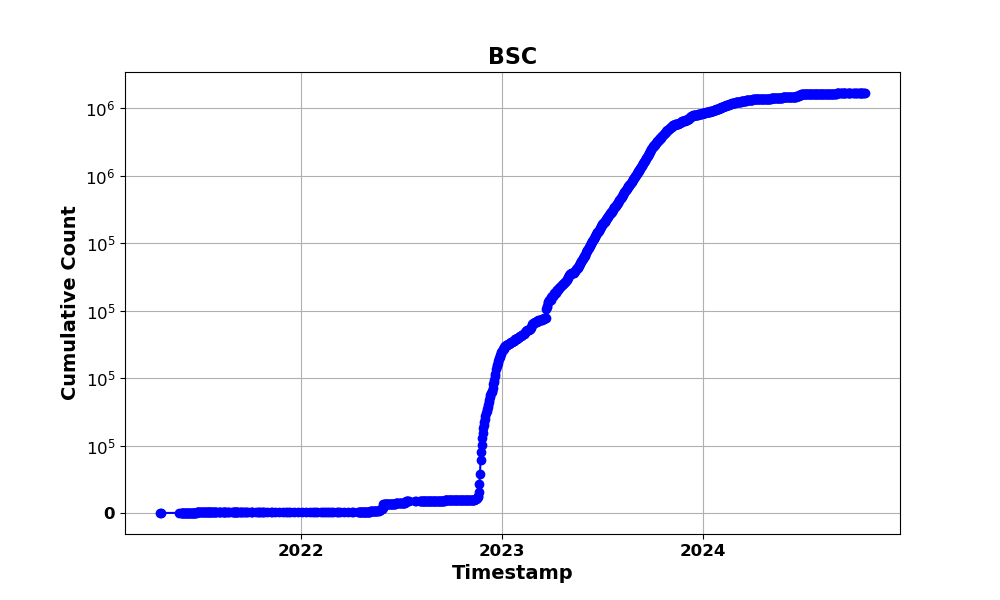
\includegraphics[width=\linewidth]{Sections/Picture/BSC.png}
        \caption{BSC}
        \label{fig:bsc}
    \end{subfigure}
    \vfill
    \begin{subfigure}[b]{\linewidth}
        \centering
        
\includegraphics[width=\linewidth]{Sections/Picture/ETH.png}
        \caption{ETH}
        \label{fig:eth}
    \end{subfigure}
    \vfill
    \begin{subfigure}[b]{\linewidth}
        \centering
        
\includegraphics[width=\linewidth]{Sections/Picture/Polygon.png}
        \caption{Polygon}
        \label{fig:polygon}
    \end{subfigure}
    \caption{针对 9 个地址在不同平台上的 ERC-20 转账幻影事件分析。}
    \label{fig:phantom_events_across_platforms}
\end{figure}

\label{sec:evaluation}
我们的工具采用 Python 实现，支持对智能合约进行字节码级和源代码级分析，同时支持交易级监控。对于字节码级分析，我们使用 Gigahorse 框架从已编译字节码中构建 ICFG。在源代码级，我们的工具支持所有与 Slither~\cite{Slither} 兼容的 Solidity 版本，使我们能够提取 AST，并对事件发出和参数约束进行详细分析。我们采用 Z3~\cite{Z3} 作为约束求解器，用于处理符号执行并消除不可行路径。此外，该工具还包含一个交易级链下监控系统，能够解析链上数据，并应用自定义规则检测异常和验证攻击交易是否成功。所有主要组件，包括字节码分析引擎、源代码符号执行器和交易监控系统，均由我们开发。该实现基于 Python，代码量超过 5,000 行。


\begin{itemize}%[leftmargin=*,topsep=2pt]
  \item \textbf{RQ1} \textit{幻影事件在主流区块链平台上有多普遍，\tool 在交易级检测中的表现如何？} 我们旨在理解验证者通过合约地址和源函数验证事件来源的必要性。
  \item \textbf{RQ2} \textit{\tool 从智能合约中检测潜在幻影事件的效果如何？} 我们开发了 \tool，并构建了一个自定义基准来评估其有效性。
  \item \textbf{RQ3} \textit{在真实世界中实施此类攻击的可行性如何？} 我们旨在验证所识别漏洞是否能够在真实场景中被实施。
\end{itemize}

\subsection{幻影事件的普遍性（RQ1）}

TokenScope~\cite{TokenScope} 等工具有助于检测代币行为中的不一致性，Guoyi Ye 等人~\cite{wallet_visual}也展示了转账事件中伪造用户地址的普遍性。我们旨在探索两个具体方面：幻影事件攻击中可疑地址的普遍性，以及此类攻击是否在跨链桥中常见。

\subsubsection{方法}

为更好地理解幻影事件在真实世界中的发生情况，我们使用区块链交易数据进行了两个独立实验。

在第一个实验中，我们重点关注九个特定伪造地址，即从 \emph{0x1111...1111} 到 \emph{0x9999...9999}，因为这些地址在正常交易中被生成或使用的可能性极低。我们检查了截至 2024 年 10 月 21 日在 Ethereum、BSC 和 Polygon 区块链上的交易，寻找源自这些地址的 ERC-20 代币转移。该方法有助于衡量不同区块链平台上幻影事件的普遍性。

在第二个实验中，考虑到跨链桥高度易受幻影事件攻击影响，我们基于交易级分析为跨链桥创建了检测规则。我们使用 XScope~\cite{Xscope} 的相关数据集，将结果与其发现进行比较；XScope 是目前唯一已有的桥攻击交易检测工具。


\subsubsection{结果}

%\begin{table}[t]
%\caption{Analysis of ERC-20 transfer phantom events across different platforms for 9 addresses.}
%\centering
%\begin{tabular}{ll}
%\toprule
%\textbf{Platforms} & \textbf{Potential Phantom Events} \\
%\midrule
%Ethereum & 18,099 \\
%BSC & 1,243,917 \\
%Polygon & 436,477 \\
%\midrule
%\textbf{Total} & \textbf{1,661,813} \\
%\bottomrule
%\end{tabular}
%\label{table:phantom_events_across_platforms}
%\end{table}



在第一个实验中，我们围绕九个特定地址进行分析，识别出 ERC-20 代币转账中存在大量幻影事件，如\cref{fig:phantom_events_across_platforms}所示。我们在 Ethereum 上发现 18,099 个此类事件，在 BSC 上发现 1,245,125 个，在 Polygon 上发现 436,407 个。如果这些事件未被适当验证，可能导致安全漏洞利用。仅九个地址就出现如此显著的事件数量，凸显了严格交易验证对于维护区块链操作安全性和可信度的关键必要性。


%\begin{table}[htbp]
%    \centering
%    \caption{Number of detected attack transactions by tools.}
%    \label{tab:attack_detection}
%    \begin{tabular}{lrr}
%        \toprule
%        \textbf{Project} & \textbf{XScope} & \textbf{\tool} \\
%        \midrule
%        THORChain \# 1 & 9 & 9 \\
%        THORChain \# 2 & 41 & 48 \\
%        pNetwork & 3 & 5 \\
%        Qubit Bridge & 20 & 20 \\
%        meter.io & N/A & 5 \\
%        CENNZnet & N/A & 1 \\
%        \bottomrule
%    \end{tabular}
%\end{table}

\begin{table}[t]
    \centering
    \caption{不同工具检测到的攻击交易数量和成功攻击数量。}
    \label{tab:attack_detection}
    \begin{tabular}{l r r r}
        \toprule
        \textbf{项目} & \textbf{XScope} & \multicolumn{2}{c}{\textbf{\tool}} \\
        \cmidrule(lr){2-2} \cmidrule(lr){3-4}
        & \textbf{攻击} & \textbf{攻击交易} & \textbf{成功攻击} \\
        \midrule
        THORChain \#1 & 9 & 9 & 9 \\
        THORChain \#2 & 41 & 48 & 41 \\
        pNetwork & 3 & 5 & 3 \\
        Qubit Bridge & 20 & 20 & 20 \\
        meter.io & N/A & 5 & 5 \\
        CENNZnet & N/A & 1 & 1 \\
        \bottomrule
    \end{tabular}
\end{table}


在第二个实验中（结果如\cref{tab:attack_detection}所示），我们检测到了 XScope 报告的所有交易，并识别出了额外的攻击交易。XScope 只记录攻击已经发生的交易，其标志是目标链上发生了资金转移。相比之下，我们能够在转账发生前检测攻击，从而帮助项目团队主动识别攻击者。我们还检测到了 meter.io~\cite{Meter} 上的攻击交易；XScope 虽然在其攻击事件列表中提到了该项目，但并未进行分析。此外，我们在 CENNZnet 上发现了一笔攻击交易，造成了 150 ETH 的损失。该事件此前未被任何其他工具或安全公司披露或报告。

\vspace{\baselineskip}
\begin{mdframed}
\noindent\textbf{对 RQ1 的回答：} \textit{我们的分析表明，仅基于九个地址，就能发现 Ethereum、BSC 和 Polygon 上存在大量幻影事件。此外，与当前先进工具相比，我们的检测规则展现出了有效性。}
\end{mdframed}

\subsection{从代码中检测幻影事件（RQ2）}

\subsubsection{数据集}
SmartAxe~\cite{liao2024smartaxe} 和 XGuard~\cite{wang2024xguard} 是目前已知的两个用于检测跨链漏洞的工具，其中 SmartAxe 侧重于字节码级分析，而 XGuard 提供源代码级分析。

在对 SmartAxe 数据集的分析中，我们发现 20 起攻击中只有 8 起由\emph{事件仿冒}导致，并且桥合约中存在存在漏洞的函数路径对。我们重新标注了这 8 起攻击，并从 SmartAxe 分析的 129 个桥中额外添加了 29 对受\emph{事件仿冒}影响的函数路径。作为补充，我们从 BSC~\cite{bscdata} 中 452,666 个已验证合约中，使用 TF-IDF 算法选择了 500 个相似度较低的 BSC 智能合约并进行人工标注。去重后，我们额外识别出 80 对受\emph{事件仿冒}影响的函数对。

通过结合 SmartAxe 和 XGuard 数据集以及人工标注的函数对，我们构建了一个综合数据集，其中包含 117 对受\emph{事件仿冒}影响的函数对，用于评估我们的检测工具。

为检测\emph{不一致日志记录}，我们使用了一个由 28 个经人工审计的不一致日志记录参数案例组成的数据集，这些案例是在我们的审计过程中识别出来的。

\subsubsection{结果}

\begin{table*}[htbp]
    \centering
    \caption{事件仿冒与不一致日志记录检测中的工具比较}
    \label{tab:tool_result}
    \small
    \begin{tabular}{p{3.9cm}ccc ccc}
        \toprule
        \multirow{2}{*}{\textbf{工具}} & \multicolumn{3}{c}{\textbf{事件仿冒}} & \multicolumn{3}{c}{\textbf{不一致日志记录}} \\
        \cmidrule(lr){2-4} \cmidrule(lr){5-7}
        & \textbf{精确率} & \textbf{召回率} & \textbf{F1} & \textbf{精确率} & \textbf{召回率} & \textbf{F1} \\
        \midrule
        SmartAxe & 40.50\% & 25.12\% & 31.01\% & N/A & N/A & N/A \\
        XGuard & 87.75\% & 55.12\% & 67.70\% & 64.71\% & 91.75\% & 75.82\% \\
        \tool (Bytecode) & 84.0\% & 100\% & 91.30\% & 62.50\% & 16.12\% & 39.31\% \\
        \tool (Source) & 90.83\% & 86.51\% & 88.62\% & 90.30\% & 100\% & 94.90\% \\
        \bottomrule
    \end{tabular}
\end{table*}
在实验中，如\cref{tab:tool_result}所示，\tool 在检测\emph{事件仿冒}和\emph{不一致日志记录}漏洞方面均显著优于 SmartAxe 和 XGuard。对于\emph{事件仿冒}，SmartAxe 的 F1 分数为 31.01\%，精确率为 40.50\%，召回率为 25.12\%；XGuard 的 F1 分数为 67.70\%，精确率为 87.75\%，召回率为 55.12\%。相比之下，\tool 表现更优，在字节码级达到 91.30\% 的 F1 分数，在源代码级达到 88.62\% 的 F1 分数。对于\emph{不一致日志记录}检测，\tool 同样优于 XGuard，在召回率达到 100\% 的情况下取得了 94.9\% 的 F1 分数，而 XGuard 的 F1 分数为 75.82\%。

\tool 的字节码级实现和源代码级实现之间的性能指标差异，凸显了两种方法各自的局限性。在\emph{事件仿冒}检测中，\tool 的字节码级分析缺乏约束验证，因此可能将缺少充分伪造证据的事件标记出来，导致精确率较低。然而，在源代码级，\tool 会执行全面的约束检查，从而显著提高精确率。对于\emph{不一致日志记录}，\tool 的字节码分析仅限于索引参数，因此无法识别与非索引参数相关的问题，进而降低召回率。在具备源代码访问权限时，\tool 可以同时分析索引参数和非索引参数，因此取得更高召回率。相比之下，SmartAxe 和 XGuard 存在固有设计限制：SmartAxe 只检测两个函数是否发出同一事件，而不考虑调用路径中的约束验证；XGuard 则关注单个函数内部的约束，缺乏函数间分析。通过同时分析函数交互和调用路径，\tool 能够检测其他工具遗漏的漏洞，并在\emph{事件仿冒}和\emph{不一致日志记录}检测中取得更优结果。


\subsubsection{局限性}

评估中的误报和漏报揭示了本文方法的两个主要局限。首先，在处理不完整合约代码时，例如某些函数中的接口调用，我们计算得到的约束未必总是精确，这会导致约束较弱并进而产生误报。其次，由于 Solidity 编译缺陷，一些已通过区块链浏览器验证的智能合约在使用我们的工具进行分析时出现编译错误~\cite{compile_issue}。解决这些局限将是我们未来工作的重点。


\vspace{\baselineskip}
\begin{mdframed}
\noindent\textbf{对 RQ2 的回答：} \textit{\tool 在检测幻影事件漏洞方面被证明高度有效，并在精确率、召回率和 F1 分数上超过了当前先进工具。}
\end{mdframed}

\subsection{真实世界攻击可行性（RQ3）}
\subsubsection{方法}
我们将工具应用于多个区块链平台进行测试，旨在识别智能合约中与幻影事件攻击相关的漏洞。除链上测试外，我们还审计了多种链下应用，包括区块链浏览器、NFT 市场和加密货币钱包。这些审计侧重于评估安全协议，并识别可能被幻影事件利用的潜在漏洞，从而确保对链上和链下组件进行全面分析。

所有已识别的幻影事件漏洞均在受控本地环境中通过模拟场景进行测试，以确保不会对真实世界区块链平台造成干扰或损害。

\subsubsection{结果}

在实验中，我们识别出一笔\emph{转账事件欺骗}交易，其中一次虚假转账看起来像是将代币从地址 \textit{0x8888...8888} 转入受害者钱包。尽管实际上并未发生任何代币转账，至少五个主要区块链浏览器 BscScan、OKLink、Bitquery、Tokenview 和 Bsctrace~\cite{bscscan,oklink,bitquery,tokenview,bsctrace} 都错误地将该欺骗事件识别为合法交易。这凸显了链下系统中的普遍脆弱性，即它们难以区分真实事件和幻影事件。

此外，我们在两个领先 NFT 市场 Opensea 和 Rarible 的测试网环境中成功复现了 ``sleepminting'' 攻击。尽管已有用于检测此类攻击的监控方案，但完全缓解这些漏洞仍是一项持续挑战。

此外，在安全审计过程中，我们在六个加密货币钱包中发现了关键漏洞，并将其报告给相应项目团队或通过漏洞赏金平台报告。其中四个漏洞已被确认，一个漏洞为我们带来了来自项目团队的 600 美元赏金。

在对多个区块链桥的审计中，我们识别出链下代码中的漏洞，使这些桥暴露于仿冒合约攻击之下。在该攻击中，恶意合约会发出伪造事件，而链下系统会错误地将其作为合法事件处理。我们发现的一个存在漏洞的系统曾被某个公链项目分叉并部署，截至 2024 年 10 月 9 日，该项目市值超过 2.5 亿美元。这些漏洞已报告给相应项目团队以便修复。


此外，我们在流行区块链浏览器 Blockscout~\cite{error_display} 中识别出一个事件数据显示问题，该问题可能损害交易记录的准确性。该缺陷可能导致用户误解区块链数据，从而削弱其对交易历史的信任。

在对多个活跃智能合约项目的审计中，我们还发现三个 DeFi 项目和一个 GameFi 项目易受\emph{不一致日志记录}攻击影响，该漏洞由本文首次提出（见\ref{vec:attack2}）。在这组项目中，受影响项目的最高市值为 169,688 美元。


\vspace{\baselineskip}
\begin{mdframed}
\noindent\textbf{对 RQ3 的回答：} \textit{我们的研究表明，幻影事件攻击在真实世界区块链平台上具有可行性，具体目标包括区块链浏览器、NFT 市场、DeFi、GameFi 和加密货币钱包。这强调了在区块链生态系统中改进安全措施的迫切需求。详细报告和确认案例可见补充材料。}
\end{mdframed}


\subsection{有效性威胁}
内部有效性威胁主要源于人工数据标注过程中可能引入的不准确性。为提高数据标注准确性，我们采用了三层方法：两名作者独立标注数据，第三名作者审查其标注结果。该方法在三个不同层级进行了彻底审查，以提高数据集分类的精确性。

为确保外部有效性，我们使实验中使用的数据集类型和来源更加多样化。除 SmartAxe 和 XGuard 提供的以桥为中心的数据外，我们还扩展了数据集，使其包含更广泛的场景。此外，我们避免使用相似度较高的智能合约，以提高分析的多样性和有效性。

\section{相关工作}
\subsection{智能合约安全分析}
近年来，大量技术被提出用于分析智能合约安全性。

\paragraph{静态分析}
Tikhomirov 等人~\cite{tikhomirov2018smartcheck}设计了 SmartCheck，该系统将 Solidity 源代码转换为 XML，并通过 xPath 模式检测缺陷。Grech 等人~\cite{grech2022elipmoc}提出了名为 Gigahorse 的静态分析框架，该框架将基于栈的字节码转换为基于寄存器的中间表示。Fesit 提出了一个面向 Solidity 源代码的类似工具 Slither~\cite{Slither}。Lu 等人~\cite{lu2021neucheck}设计了名为 NeuCheck 的智能合约安全分析工具，该工具基于语法树解析。Ghaleb 等人~\cite{ghaleb2022etainter}提出了 eTainter，这是一种静态分析工具，通过将污点追踪应用于字节码来检测智能合约中的 gas 相关漏洞。

\paragraph{符号执行}
Luu 等人~\cite{luu2016making}提出了 Oyente，这是一个用于检测 Ethereum 智能合约缺陷的开创性符号执行工具。Lin 等人~\cite{lin2022solsee}提出了 SolSEE，这是首个面向 Solidity 智能合约的源代码级符号执行引擎。Ma 等人~\cite{ma2021pluto}提出了 Pluto，通过重建合约间 CFG 来检测安全缺陷。Pasqua 等人~\cite{pasqua2023enhancing}提出了一种基于 EVM 操作数符号执行的方法，用于精确构建 CFG 并改进漏洞检测。Ruaro 等人~\cite{ruaro2024not}实现了 CRUSH，该工具利用符号执行和程序切片检测此类合约组之间的存储冲突。Gritti 等人~\cite{gritti2023confusum}开发了 JACKAL，该工具基于控制流图（CFG）和函数调用图（FCG）执行符号执行，以检测混淆合约漏洞。此外，Mytrhil~\cite{mythril} 和 Manticore~\cite{mossberg2019manticore} 等工业界解决方案已成为智能合约审计的标准工具。

我们的方法是开发一个结合多种技术的检测框架，包括字节码级分析、源代码分析、交易级监控和符号执行；但本文所处理的问题无法被任何现有漏洞模式捕获。

\subsection{智能合约事件}
通常而言，日志消息能够增强程序理解并降低维护成本，但关于 Solidity 事件日志记录和安全性的研究仍然有限。Li 等人~\cite{li2023understanding}首次对 Solidity 事件日志记录开展了实证研究，并开发了一种工具，用于识别会造成不必要 gas 消耗的事件。Zhang 等人~\cite{Xscope}设计了名为 Xscope 的工具，用于发现跨链桥中的安全违规事件。Cernera 等人~\cite{cernera2023token}通过扫描日志并查找 Transfer 事件，追踪由内部交易创建的代币。此外，Guidi 等人~\cite{sleepminting}分析了 sleepminting 现象，并探索了使用 Forta 追踪可疑事件和发出告警的方法。Zhu 等人~\cite{doccon}提出了名为 DocCon 的技术，用于检测 Solidity 代码及其对应文档之间的不一致。这些不一致包括文档中记录的事件发出行为未出现在代码中，或代码中出现了文档未记录的事件发出行为。TokenScope \cite{TokenScope} 通过监控 ERC-20 事件，为检测代币行为中的不一致性作出了贡献。尽管已有这些进展，大多数研究仅考虑了特定场景中与事件相关的问题，尚未充分解决由幻影事件导致攻击的一般性问题。

\label{sec:related}

\section{缓解策略}
\label{sec:mitigation}

缓解由幻影事件导致的漏洞需要采用综合方法，覆盖智能合约开发、生态基础设施以及攻击检测机制。从合约开发角度看，开发者应实现严格的验证机制，以确保事件参数在发出前经过验证，并为相关函数设置访问控制机制。强制执行适当的状态转换同样至关重要，这可以防止发出的事件与实际合约状态之间出现不匹配。

在生态系统层面，区块链浏览器、钱包和 DApp 等链下系统必须采用更稳健的验证技术，以区分合法事件和幻影事件。事件发出者验证通过将事件来源与合约地址进行交叉检查，有助于确保事件源自被授权合约。此外，改进链下应用中的数据清理流程对于防止跨站脚本（XSS）和 SQL 注入（SQLi）等漏洞至关重要。对于跨链桥而言，还需要增强跨链安全协议，确保源链和目标链上的事件都经过验证，以防止事件伪造和操纵。

在安全攻击检测方面，对链上交易和事件进行持续实时监控对于检测并标记可疑活动至关重要，例如\emph{转账事件欺骗}或\emph{合约仿冒}。针对链上合约行为和链下事件处理分别定义详细检测规则，有助于更全面地识别漏洞。此外，应定期对智能合约和链下系统进行安全审计，以识别潜在弱点，尤其应关注事件发出逻辑、访问控制和交易验证。通过综合运用这些策略，可以显著降低幻影事件带来的风险，并提高区块链系统的安全性和可靠性。

\section{结论}

本文对区块链系统中与幻影事件相关的漏洞进行了深入分析。我们开发了一个多层级检测框架，集成字节码级、源代码级和交易级分析，以处理\emph{事件仿冒}、\emph{不一致日志记录}和\emph{合约仿冒}等问题。此外，我们为所提出的每一种攻击向量都识别出了真实世界案例，凸显了在区块链生态系统中缓解这些威胁的关键必要性。



\input{Sections/Acknowledgments}

\input{bibliography}
\appendices

%\section{Attack Sequence of pNetwork Hack}

%\Cref{fig:sqeuence} shown the attack sequence of pNetwork attack.
%\label{pnetwork_sequence}
\section{真实世界攻击示例}

\subsection{本文分类中五类攻击向量的示例}
\label{appendix:examples}

\paragraph{事件仿冒}
\emph{事件仿冒}的两个知名实例是针对 Qubit Bridge~\cite{Qubit} 和 Meter Bridge~\cite{Meter} 的攻击，分别造成了 8000 万美元和 430 万美元的损失。

\paragraph{不一致日志记录}
许多此类问题是在 2024 年 4 月 1 日对 BSC 链上最活跃的 25 个智能合约进行分析时发现的。具体而言，TroyEmpire~\cite{TroyEmpire}、SecondLive~\cite{SecondLive}、WalletLocking~\cite{WalletLocking} 和 TTGameEvents~\cite{TTGame} 的合约被发现存在这些问题。例如，TTGame 项目会为用户注册生成一个地址，并向该地址转入一定数量的 BNB，作为未来自动调用所需的 gas 费用。通过从历史交易中识别授权用户地址，我们可以发现其余发出幻影事件的未授权交易。尽管其他三个项目的用户权限并不明确，但我们可以通过模拟调用它们的函数任意生成取款事件，从而确认这些问题的存在。

\paragraph{合约仿冒}
对于\emph{合约仿冒}攻击，最显著的实例是针对 pNetwork 的攻击，该攻击造成了 1270 万美元损失。该案例已在\cref{sec:motivation}中作了简要介绍。类似地，THORChain 也因错误处理器问题遭受了 800 万美元损失~\cite{thorchain}。至于仿冒合约攻击，一个代表性案例是 ``sleepminting'' 攻击，该攻击因生成一个价值 6900 万美元的 NFT 并将其上架到平台而受到关注。该事件已在学术界得到广泛研究~\cite{nft_sleepminting,clone_nft,sleepminting}。根据 Forta 平台近期信息~\cite{sleepminting_forta}，在 2023 年 12 月 3 日至 12 月 9 日短短 7 天内，就生成了 8,130 条 sleepminting 告警。

\paragraph{转账事件欺骗}
我们对链上数据的分析揭示了大量\emph{转账事件欺骗}实例，其中 ERC-20 代币和 NFT 事件的发送者地址被篡改。这些实例包括类似名人、知名交易所和其他吸引注意力实体的伪造地址。其中若干案例已导致重大经济损失~\cite{layerzero_scam,TetherClaims,ethaddress,zero_transfer,wallet_visual}。

\paragraph{事件处理错误}
\emph{事件处理错误}的一个知名示例是 Rarible 和 OpenSea 因 sleepminting 遭遇的错误信息展示案例。Etherscan 和 Bscscan 等区块链浏览器以及各种钱包，常常会将伪造转账事件视为合法交易。另一个实例涉及 blockwell.ai，其中钱包错误地将来自欺骗代币的幻影事件识别为有效 ERC-20 转账~\cite{blockwell.ai}。在 ERC-721 和 ERC-1155 代币中也观察到了类似漏洞。

此外，最大的 NFT 市场 OpenSea 也曾面临类似问题。攻击者操纵 OpenSea 所显示 NFT 的元数据，并嵌入恶意载荷以触发非预期的钱包行为，最终使攻击者获利。类似攻击也出现在 ERC-20 项目中，这凸显了整个区块链生态系统在安全处理事件数据方面所面临的普遍困难~\cite{rektosaurus,OpenSea}。

\subsection{不一致日志记录与合约仿冒框架}

\begin{figure}
    \centering
    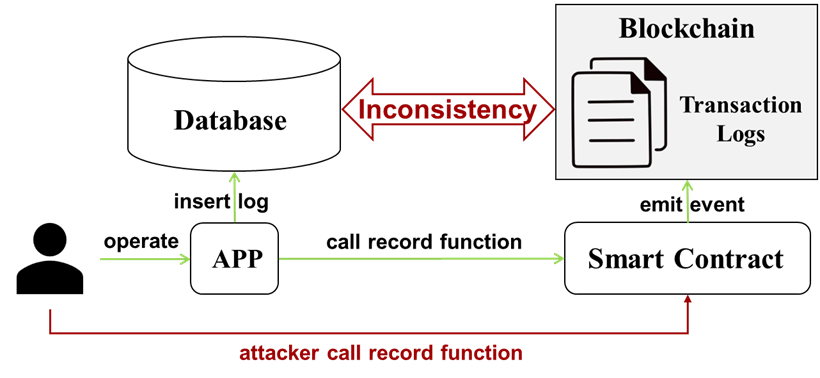
\includegraphics[width=1\linewidth]{Sections//Picture/inconsistency.png}
    \caption{不一致日志记录应用概览。}
    \label{fig:Inconsistent_logging}
\end{figure}

~\Cref{fig:Inconsistent_logging} 给出了应用中\emph{不一致日志记录}的概览。在该框架中，用户通过应用进行操作，应用一方面与数据库交互以插入日志，另一方面与区块链上的智能合约交互以发出事件。然而，由于日志记录实践存在差异，数据库日志和区块链交易日志之间可能出现不一致。攻击者可以通过直接调用记录函数来利用这一点，从而可能在应用内部日志记录与区块链交易日志之间制造不匹配。

\begin{figure}[!htbp]
    \centering
    \begin{subfigure}[b]{0.5\textwidth}
        \centering
        
\includegraphics[width=\textwidth]{Sections/Picture/attack1-1.png}
        \caption{混合事件攻击}
        \label{fig:attack3-1}
    \end{subfigure}
    \quad
    \begin{subfigure}[b]{0.5\textwidth}
        \centering
        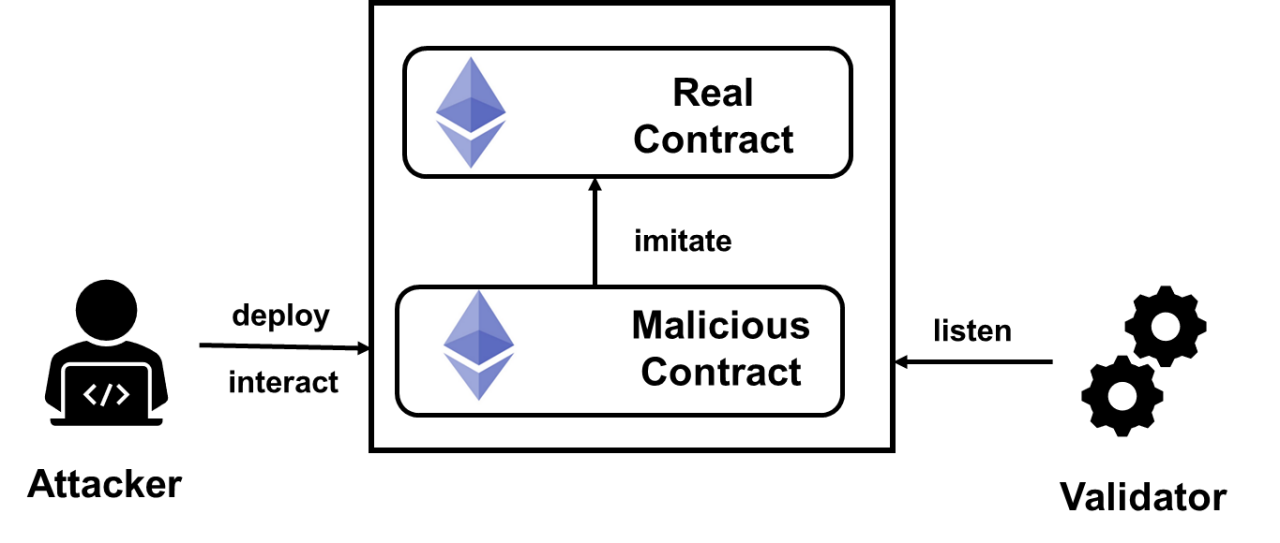
\includegraphics[width=\textwidth]{Sections/Picture/attack1-2-0.png}
        \caption{仿冒合约攻击}
        \label{fig:attack3-2}
    \end{subfigure}
    \caption{两类合约仿冒}
    \label{fig:attack1}
\end{figure}

~\Cref{fig:attack1} 展示了两类合约仿冒攻击。在\emph{混合事件攻击}中，恶意合约与真实合约交互，两个合约的日志被记录在同一笔交易中，这可能误导验证者。在\emph{仿冒合约攻击}中，攻击者部署一个模仿真实合约的合约，生成看似源自真实合约的欺骗性日志，进一步干扰验证者判断。

\subsection{转账事件欺骗案例}

\begin{figure}
    \centering
    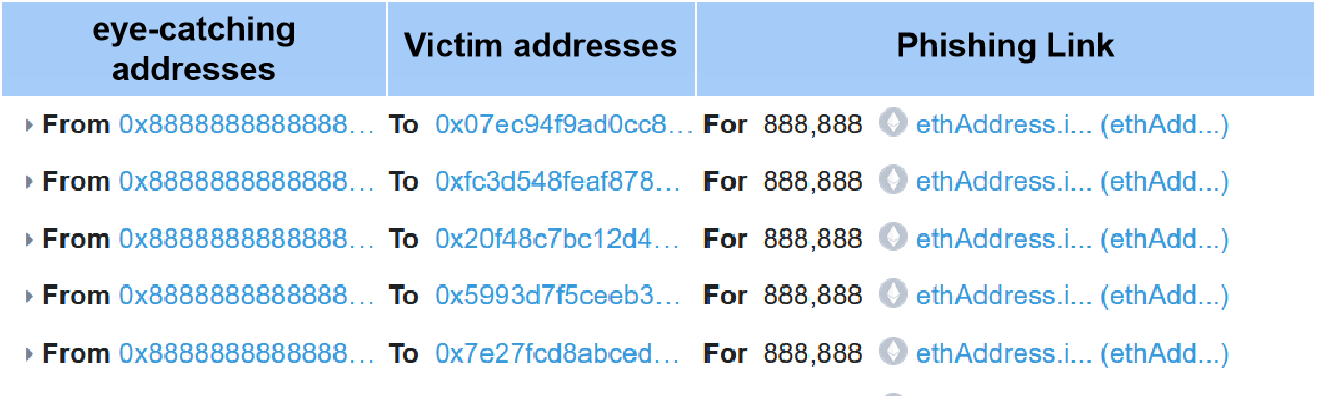
\includegraphics[width=1\linewidth]{Sections//Picture/address.png}
    \caption{空投事件欺骗。}
    \label{fig:airdrop}
\end{figure}

~\Cref{fig:airdrop} 展示了一个\emph{转账事件欺骗}攻击示例，其中攻击者伪造事件发送者，导致区块链浏览器和钱包错误地将其显示为一次成功转账。这种错误展示可能欺骗用户，并被用作一种社会工程学手段，以利用用户对这些界面的信任。


% \section{Real case of transfer event spoofing attack transactions.}
\begin{table}[]
\caption{转账事件欺骗攻击交易的真实案例。}
\label{tab:transfer_spoof_attack_transaction}
\begin{tabular}{lllll}
\toprule
  & 发送者 & 转账来源                & 转账去向                  & 代币      \\
\midrule
1 & Victim           & Victim & 0x{\color[HTML]{FE0000}734}659...50C{\color[HTML]{FE0000}a79F7} & USDT \\
\midrule
2 & Attacker              & Victim & 0x{\color[HTML]{FE0000}734}35A..2Bc{\color[HTML]{FE0000}a79F7}  & FAKE USDT     \\
\midrule
3 & Victim           & Victim & 0x{\color[HTML]{FE0000}734}35A...2Bc{\color[HTML]{FE0000}a79F7} & USDT \\
\bottomrule
\end{tabular}
\end{table}
2024 年 2 月 9 日发生的\emph{转账欺骗}攻击中，攻击者成功执行了一次\emph{转账事件欺骗}攻击，造成 104 万美元损失。该攻击利用了钱包和区块链浏览器在解析和显示转账事件时存在的漏洞。如\Cref{tab:transfer_spoof_attack_transaction}所示，在用户向合法地址（0x734\ldots{}a79F7）发送资金后，攻击者伪造了一个转账事件，使其看起来像是资金被发送到了一个由攻击者控制的相似地址。由于某些钱包和浏览器处理这些事件的方式存在问题，该虚假转账被显示为合法交易，导致用户误将额外资金发送到攻击者地址，造成重大经济损失~\cite{zero_transfer}。


\end{document}
